\documentclass[a4paper]{article}

\usepackage[top=2cm, bottom=2cm, left=3cm, right=3cm]{geometry}

\usepackage{float}

\usepackage{multirow}

\usepackage[hyphens]{url}
\usepackage{hyperref}

\usepackage{appendix}
\usepackage[numbers]{natbib}

\usepackage{graphicx}

\newcommand{\mytilde}{\raise.17ex\hbox{$\scriptstyle\mathtt{\sim}$} }


% For \begin{acknowledgements}
% From: http://www.latex-community.org/forum/viewtopic.php?f=47&t=5464
\makeatletter
\newcommand\ackname{Acknowledgements}
\if@titlepage
  \newenvironment{acknowledgements}{%
      \titlepage
      \null\vfil
      \@beginparpenalty\@lowpenalty
      \begin{center}%
        \bfseries \ackname
        \@endparpenalty\@M
      \end{center}}%
     {\par\vfil\null\endtitlepage}
\else
  \newenvironment{acknowledgements}{%
      \if@twocolumn
        \section*{\abstractname}%
      \else
        \small
        \begin{center}%
          {\bfseries \ackname\vspace{-.5em}\vspace{\z@}}%
        \end{center}%
        \quotation
      \fi}
      {\if@twocolumn\else\endquotation\fi}
\fi
\makeatother

\title{Towards Debugging Wireless Sensor Network Applications}
\date{October 2012 - July 2013}
\author{}

\begin{document}

\maketitle

%No numbering on first and second pages
\pagestyle{empty}
\thispagestyle{empty}

\newpage

\begin{abstract}
Abstract
\newline
\newline
\noindent \textbf{Keywords} - Keywords;
\end{abstract}
\newpage

\begin{acknowledgements}
Acknowledgements
\end{acknowledgements}
\newpage


\pagestyle{plain}
\setcounter{page}{1}

\tableofcontents
\clearpage


\section{Introduction}

Wireless sensor networks (WSNs) are becoming increasing prevalent due to decreasing hardware cost and hardware size \cite{TankBible}. Therefore, it is important that we consider issues with them now, so we are prepared for when they become widely used. A major issue with any system is that it may contain bugs, fortunately, there are many well known methodologies for detecting and eliminating bugs \cite{1382572, 749477, ?}. However, in distributed systems there are additional challenges to overcome \cite{5010224} and there are additional challenges to overcome with WSNs due to the energy constrained environment they work in \cite{?}.

\clearpage


\section{Knowledge Gained}
\begin{enumerate}
	\item Not possible to write WSN applications in Java and have them run on the WSN nodes. Only possible to write in C and have that code run on the physical hardware. Java code will only run in the Cooja simulator for the Contiki OS.
	\item A Cooja plug-in that monitors and records network traffic would be specific only to the simulator and would not be possible to apply to physical nodes
\end{enumerate}
\clearpage


\section{Project Management}

\subsection{Work Overview}

% TODO: Convert this to a table that can flow over multiple pages
\begin{table}[H]
	\centering
	\begin{tabular}{| l | p{7.5cm} | p{5cm} |}
	Week & Activities & Task Allocation\\
	\hline
	1 & \begin{enumerate}
			\item Met up with Supervisor and discussed project direction
			\item Decided to research what has been done and what we could do, before settling on main aims
			\item Investigated two OSes and their corresponding simulators TinyOS with TOSSIM and Contiki with Cooja
		\end{enumerate} &
	\begin{enumerate}
		\item[] Amit: 1, 2, 3
		\item[] Dan: 1, 2, 3
		\item[] Ivan: 1, 2, 3
		\item[] Joe: 1, 2, 3
		\item[] Matt: 1, 2, 3
		\item[] Tim: 1, 2, 3
	\end{enumerate}
	\\ \hline

	2 & \begin{enumerate}
			\item Research if Cooja can be extended through the use of plug-ins (with the aim of extending it to replay traffic logs)
			\item Research Clustering algorithms and find implementations
			\item Develop a temperature dissemination application to learn Contiki and Cooja
			\item Research TinyOS and TinyDB and see if they could be applied to predicate checking
			\item Investigate performance of different MAC protocols
			\item Investigate the feasibility of live monitoring of the network
			\item Investigate QoS and how it may be applied to real life WSN deployments
			\item Produce a literature review on chosen topic
		\end{enumerate} &
	\begin{enumerate}
		\item[] Amit: 1, 7, 8
		\item[] Dan: 5, 8
		\item[] Ivan: 6, 8
		\item[] Joe: 4, 8
		\item[] Matt: 3, 8
		\item[] Tim: 2, 8
	\end{enumerate}
	\\ \hline

	\end{tabular}
\end{table}

\subsection{Role Allocation}

We decided to allocate roles in the second week after we had the first week to perform research into the problem and find out what has been done. The following were how we assigned roles, although we intend for these to be flexible:

\begin{table}[H]
	\centering
	\begin{tabular}{| l | l |}
	Name & Role \\
	\hline
	Amit & ~ \\
	Dan & ~ \\
	Ivan & ~ \\
	Joe & ~ \\
	Matt & ~ \\
	Tim & ~ \\
	\end{tabular}
\end{table}


\subsection{Schedule}


\begin{table}[H]
	\centering
	\begin{tabular}{| l | l |}
	Task Description & Time Allocation \\
	\hline
	\hline
	\multicolumn{2}{|l|}{\textbf{Term 1}} \\
	\hline

	Research around the Problem & 1 Week \\
	Writing Specification & 0.5 Weeks \\
	Algorithm Development & 3 Weeks \\
	Testing on Physical Nodes & 2 Weeks \\

	\textbf{TODO!!!} & 3 Weeks \\

	Poster Creation and Presentation preparation & 0.5 Weeks \\

	\hline
	\hline
	\multicolumn{2}{|l|}{\textbf{Term 2}} \\
	\hline

	\textbf{TODO!!!} & 5 Weeks \\

	Testing & 3 Weeks \\
	Report Writing & 2 Weeks \\
	
	\end{tabular}
\end{table}



\subsection{Working Concurrently}

We signed up for a Git repository on BitBucket \cite{?} where we plan to commit all the work we produce. We initially had an issue that free private repositories hosted on BitBucket have a maximum of 5 participants, whereas we had 6 group members. Fortunately when new users sign up to the services from an invite, the person that sends the invite gets additional capacity. This meant that the person who created the repository ended up with enough capacity for all members to access the account.

\subsection{Group Members Without Internet}
Unfortunately two of our group members were without internet for the first 3 weeks of term. This was an issue because they were unable to just work in the DCS labs because the computers there didn't have the software required (such as VirtualBox or the WSN simulators). To work around this, those two members were given tasks that could be accomplished with their own machines and without internet. Once they obtained internet they were given tasks that, that access allowed them to acomplish.

\clearpage

\appendixpage
\addappheadtotoc
\appendix

\section{Device Specifications}

\subsection{Sensor Board: CM5000}

\begin{figure}[H]
\centering
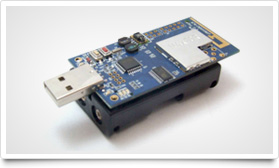
\includegraphics[scale=0.5]{Images/CM5000}
\end{figure}

\begin{table}[H]
	\centering
	\begin{tabular}{| l | l | l |}
	\hline
	\textbf{Item} & \textbf{Specification} & \textbf{Description} \\
	\hline
	\hline

	\multicolumn{3}{|l|}{\textbf{Processor}} \\
	\hline
	Processor Model & Texas Instruments\textregistered MSP430F1611 & Texas Instruments\textregistered MSP430 family\\
	\hline
	\multirow{3}{*}{Memory} & 48KB & Program Flash \\
	~ & 10KB & Data RAM \\
	~ & 1MB & External Flash (ST\textregistered M25P80) \\
	\hline
	ADC & 12bit resolution & 8 channels \\
	\hline
	\multirow{2}{*}{Interfaces} & UART, SPI, I2C & Serial Interfaces \\
	~ & USB & External System Interface (FTI\textregistered FT232BM) \\
	\hline
	\hline

	\multicolumn{3}{|l|}{\textbf{Radio}} \\
	\hline
	RF Chip & Texas Instruments\textregistered CC2420 & IEEE 802.15.4 2.4GHz Wireless Module\\
	\hline
	Frequency Band & 2.4GHz \mytilde 2.485GHz & IEEE 802.15.4 compliant \\
	\hline
	Sensitivity & -95dBm typ & Receive Sensitivity \\
	\hline
	Transfer Rate & 250Kbps & IEEE 802.15.4 compliant \\
	\hline
	RF Power & -25dBm \mytilde 0dBm & Software Configurable \\
	\hline
	Range & \mytilde120m (outdoor), 20\mytilde30m (indoor) & Longer ranges possible with optional SMA antenna attached \\
	\hline
	\multirow{3}{*}{Current Draw} & RX: 18.8mA & \multirow{3}{*}{Lower RF Power Modes reduce consumption} \\
	~ & TX: 17.4mA & ~ \\
	~ & Sleep mode: 1uA & ~ \\
	\hline
	RF Power Supply & 2.1V \mytilde 3.6V & CC2420 Input Power \\
	\hline
	Antenna & Dipole Antenna / PCB Antenna & Additional SMA connector available for extra antenna \\
	\hline
	\hline

	\multicolumn{3}{|l|}{\textbf{Sensors}} \\
	\hline
	Light 1 & Hamamatsu® S1087 Series & Visible Range (560 nm peak sensitivity wavelength)\\
	\hline
	Light 2 & Hamamatsu® S1087 Series & Visible \& Infrared Range (960 nm peak sensitivity wavelength)\\
	\hline
	\multirow{6}{*}{Temperature \& Humidity} &  \multirow{6}{*}{Sensirion® SHT11} & Temperature Range: -40 \mytilde 123.8 $^\circ$C  \\
	~ & ~ & Temperature Resolution: $\pm$ 0.01 (typical) \\
	~ & ~ & Temperature Accuracy: $\pm$ 0.4 $^\circ$C (typical) \\
	~ & ~ & Humidity Range: 0 \mytilde 100\% RH \\
	~ & ~ & Humidity Resolution: 0.05 (typical) \\
	~ & ~ & Humidity Accuracy: $\pm$ 3 \%RH (typical) \\
	\hline

	\end{tabular}
	\caption{Specifications for the CM5000 Wireless Sensor Node \cite{CM5000}}
	\label{tab:CM5000-spec}
\end{table}

\clearpage


\subsection{Interface Module: USB1000}

\begin{figure}[H]
\centering
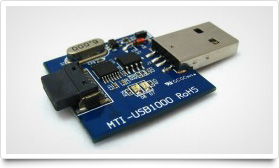
\includegraphics[scale=0.5]{Images/USB1000}
\end{figure}

\begin{table}[H]
	\centering
	\begin{tabular}{| l | l | l |}
	\hline
	\textbf{Item} & \textbf{Specification} & \textbf{Description} \\
	\hline
	\hline

	\multicolumn{3}{|l|}{\textbf{Components}} \\
	\hline
	Interface Type & USB type A & USB 1.1 compatible. USB full speed support (12Mbps)\\
	\hline
	USB2UART Chip & FTDI\textregistered FT232BM & USB2UART converter chip\\
	\hline
	1kbit EEPROM & Microchip® 93C46 & Driver ID storage\\
	\hline
	Quad Buffer & Texas Instruments\textregistered SN74HC126 & USB Rx/Tx Communications buffer\\
	\hline
	Octal Switch & Analog Devices\textregistered ADG715 & Reset sequence recognition\\
	\hline
	Mote Interface & Terminal Block (ERNI\textregistered compatible) & Connector to CMXX00 WSN Motes (Vcc, GND, 8 port ADC, 2 port GPIO pins)\\
	\hline

	\end{tabular}
	\caption{Specifications for the USB1000 Interface Board \cite{USB1000}}
	\label{tab:USB1000-spec}
\end{table}

\clearpage

\subsection{Network Infrastructure: UD1000}

\begin{figure}[H]
\centering
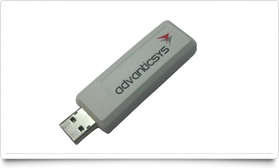
\includegraphics[scale=0.5]{Images/UD1000}
\end{figure}

\begin{table}[H]
	\centering
	\begin{tabular}{| l | l | l |}
	\hline
	\textbf{Item} & \textbf{Specification} & \textbf{Description} \\
	\hline
	\hline

	\multicolumn{3}{|l|}{\textbf{Processor}} \\
	\hline
	Processor Model & Texas Instruments\textregistered MSP430F1611 & Texas Instruments\textregistered MSP430 family\\
	\hline
	\multirow{2}{*}{Memory} & 48KB & Program Flash \\
	~ & 10KB & Data RAM \\
	\hline
	ADC & 12bit resolution & 8 channels \\
	\hline
	\multirow{2}{*}{Interfaces} & UART, SPI, I2C & Serial Interfaces \\
	~ & USB & External System Interface (FTI\textregistered FT232BM) \\
	\hline
	\hline

	\multicolumn{3}{|l|}{\textbf{Radio}} \\
	\hline
	RF Chip & Texas Instruments\textregistered CC2420 & IEEE 802.15.4 2.4GHz Wireless Module\\
	\hline
	 Frequency Band & 2.4GHz \mytilde 2.485GHz & IEEE 802.15.4 compliant \\
	\hline
	Sensitivity & -95dBm typ & Receive Sensitivity \\
	\hline
	Transfer Rate & 250Kbps & IEEE 802.15.4 compliant \\
	\hline
	RF Power & -25dBm \mytilde 0dBm & Software Configurable \\
	\hline
	Range & \mytilde40m (outdoor), 15\mytilde20m (indoor) & Dongle orientation dependant \\
	\hline
	\multirow{3}{*}{Current Draw} & RX: 18.8mA & \multirow{3}{*}{Lower RF Power Modes reduce consumption} \\
	~ & TX: 17.4mA & ~ \\
	~ & Sleep mode: 1uA & ~ \\
	\hline
	RF Power Supply & 2.1V \mytilde 3.6V & CC2420 Input Power \\
	\hline
	Antenna & Ceramic antenna & ~ \\
	\hline
	\hline

	\multicolumn{3}{|l|}{\textbf{Electromechanical Characteristics}} \\
	\hline
	Dimensions & 65mm x 22.5mm x 14mm & Including housing\\
	\hline
	Weight & 15g & ~\\
	\hline
	Power & 5V  & DC over USB\\
	\hline
	Current & 90mA  & Max rated current over USB\\
	\hline
	Operating Temperature & -25$^\circ$C \mytilde +60$^\circ$C & ~\\
	\hline
	Storage Temperature & -40$^\circ$C \mytilde +60$^\circ$C & ~\\
	\hline
	Operating Humidity & 5\% \mytilde 95\% & Non condensing\\
	\hline
	Protection type & IP20 & Non condensing\\
	\hline

	\end{tabular}
	\caption{Specifications for the UD1000 Sensor Network Sink \cite{UD1000}}
	\label{tab:UD1000-spec}
\end{table}

\newpage

\section{References}
\renewcommand{\refname}{\vspace{-1cm}}
\bibliographystyle{myplainnat}
\bibliography{../References/references}

\end{document}
